\documentclass[oneside]{ctuthesis}

\ctusetup{
	xdoctype = B,
	xfaculty = F3,
	mainlanguage = english,
	titlelanguage = english,
	title-english = {Improving Online Continual Learning with Memory Mechanisms under Non-i.i.d. Data Streams},
	title-czech = {Sázení uranu},
	department-english = {Department of Cybernetics},
	author = {Jakub Dorfman},
        keywords-english = {Bachleor Thesis, Machine Learning, Online Continual Learning},
        keywords-czech = {Bakalářská Práce, Strojové Učení, Online Continual Learning},
	supervisor = {Mgr. Jan Šochman, PhD},
	supervisor-address = {KN-G203 \\ Karlovo namesti 13 \\ 121 35, Praha 2},
	month = 5,
	year = 2025,
}

\usepackage{graphicx}
\usepackage{subcaption}
\usepackage{tikz}
\usetikzlibrary{arrows.meta, positioning}
\usepackage[ruled,vlined,linesnumbered,noend]{algorithm2e}
\usepackage{xcolor}
\usepackage{caption}
\usepackage{booktabs}
\usepackage{multirow}
\usepackage[table]{xcolor}

\ctuprocess




\begin{abstract-english}
Online Continual Learning (OCL) aims to improve the biological plausibility of machine learning models by enabling them to learn sequentially in a non-Independent and Identically Distributed stream of data. This paper follows in the notion of biological plausibility by adding three challenging and typically optional constraints to OCL. Those being a batch size of one, a finite memory size and a strict no knowledge of stream characteristics policy. These changes, if anything, make it harder to solve the most prominent problem in OCL, called catastrophic forgetting. Catastrophic forgetting manifests itself as the inability for a model trained through the typical machine learning process to perform well on any problem that is not currently.

This work chooses three methods(GSS, ER and DER++) and conducts an empirical study, to understand the intricacies of each of them. It compares how they manage their memory, how they transform the stream of data and how they they try to mitigate catastrophic forgetting.
These experiments then inspire three proposed additions to the field of OCL. First the Weave order for a dataset to increase it's non-independence. Then a method of mixing data from memory into the stream to make it more i.i.d. Lastly a successful implementation of a pre-trained embedding model into the process. 
\end{abstract-english}

\begin{abstract-czech}
TODO Prelozit abstrakt a zkontrolovat ho

Domluvit se jestli pojmenovat metodu, posleze zkontrolovat text aby souhlasil s rozhodnutim

Zkontrolovat Related Work, pridat par jinym metod, hlavne do Replay
Z toho pak pridat nekonec tabulku, ktera ze vsech poznamenanych vyfiltruje GSS, DER++, ER...

Prepsat Methods

Zkontrolovat you, would a tychle slova

ctrl-F TODO!!! konec
precist cely po sobe

Pripravit kod
Pridat zadani prace
acknowledgments
Podepsat prohlaseni o tom ze jsem to delal ja a ze jsem vyuzil ai
\end{abstract-czech}

\begin{document}

\maketitle
\chapter{Introduction}

The typical setting in machine learning, is to create a dataset with a multitude of independent and identically distributed (i.i.d.) examples. Train a model and deploy it as a static, non changing part of a program. This process has been found to be very successful in many areas~\cite{usesOfAI} but is not the way humans learn~\cite{Sigman7585}.

Human learning comes with benefits such as, not requiring huge amounts of examples to learn what an object is or that learning from non-i.i.d. data is not much of a problem~\cite{PARISI201954} for us. Also we are not static agents as we learn continually and have the ability to remember information given to us years ago. 

The field trying to bridge this gap between typical machine learning and evolution's counterpart is called continual learning~\cite{clsurvey}. It exchanges the dataset for a sequence of tasks with different distributions of data and allows the model access to only one task at a time. A subfield of continual learning that this paper is interested in is called Online Continual Learning (OCL)~\cite{oclsurvey_graphs}, which adds a constraint of allowing only a single pass over the data stream. 
The reason we chose OCL is that it has an added benefit of it being more biologically plausible than base continual learning. To make it even more biologically plausible we impose three typically optional constraints:
\begin{enumerate}
    \item A finite memory size, this is inspired by the existence of a finite sized short term memory in the human brain~\cite{VALLAR200114049}. 
    \item Batch size of one, which comes again from the human way of learning sequentially more than in parallel~\cite{Sigman7585}. 
    \item A no knowledge of stream characteristics policy. I.e. when distributions change, what the current distribution is...
\end{enumerate}

The most prominent challenge in continual learning and OCL is catastrophic forgetting~\cite{clsurvey}. It is caused by the data distribution changing with each task, which has the adverse effect of the optimization problem shifting throughout training. Leading to the model's performance on older tasks to degrade, as there is no inherent mechanism to combat re-writing the parts of the model responsible for good performance on previous tasks. 

Ways of combating catastrophic forgetting include, adding a memory module that helps to stabilize the optimization shift by remembering examples from older tasks and mixing them in to the stream that the model trains from. Another method is to add regularization terms to penalize the model for re-writing itself thus balancing old and new tasks~\cite{clsurvey}. Or to have different parts of the model in charge of different tasks, either through dynamic allocation or parameter isolation.

Through this thesis we want to familiarize ourselves with the intricacies of this problem and learn about what state of the art methods exist. Then to pick a subset of these methods, implement them, understand their shortcomings and through modifications, increase their performance. Additionally We want to create a scenario (stream) where these state of the art methods fail, and to push the field further.

To address the goals set above, this thesis conducts an empirical investigation to gauge the effectiveness and limitations of three state of the art OCL methods. Building on this foundation we make the following contributions:
\begin{itemize}
    \item A empirical study of three common OCL baselines, being Gradient Sample Selection (GSS), Experience Replay (ER) and (DER++)
    \item A novel method for mixing data from memory into the training stream, aimed at balancing the stream's class distribution and increasing the variety of examples through augmentations.
    \item A integration of a strong self-supervised visual embedding model called DINOv2~\cite{DINOv2} to simplify the classification problem. Thus creating a viable model for use in real world scenarios.
    \item A biologically plausible dataset for OCL that is constructed from small clusters(threads) of examples based on their distance in the DINOv2 embedding space.
\end{itemize}

These contributions aim to deepen the understanding in challenging OCL scenarios and to provide insites and tools for developing better models. 

\chapter{Related Work}
As the interest in this challenge has boomed in recent years, there are many methods that try to tackle OCL~\cite{oclsurvey_graphs}, The ones that make use of a some kind of memorization can, for the better part be separated into three main approaches. A regularization based approach, an architecture based approach and a replay based approach.

\section{Regularization}
The regularization based approach mitigates catastrophic forgetting by remembering an old version of the model and using it to add regularization terms to balance out the old/new data's effect on the model's training. This subcategory contains methods such as Elastic Weight Consolidation~\cite{EWC} that penalizes the models weights for changing or Learn without Forgetting~\cite{LwF} that uses the old models prediction to calculate a distillation loss for the new model. Another method that falls into this category is Dark Experience Replay++ (DER++)~\cite{DER}, but instead of remembering an old model it remembers the models prediction when it encountered a sample, so it could also be regarded as a Replay based method

\section{Architecture}
Architecture based approaches tackle catastrophic forgetting by allocating different parts of the model to different tasks, this is motivated by the notion that shared parameters create inter-task interference~\cite{clsurvey}, leading to their subsequent overwriting.
One of the methods that belong to this category is Hard-Attentions-to-the-Task~\cite{HAT} which creates a dynamic mask based on the importance of each connection to the end result. Another method that falls into this category is Winning Sub-Network~\cite{WSN}. This method dynamically reuses sub networks inside itself and freezes the networks, not currently in use.

\section{Replay}
The idea motivating all of the Replay methods is to eliminate catastrophic forgetting by transforming the non i.i.d. stream into a more typical one, that allows the model the ability to perform/learn better. This is mostly accomplished by adding a memory module that transforms the incoming stream, by mixing in examples  from itself, thus transforming it and stabilizing it's class distribution. The memory modules used, fall into one of three categories:

\textbf{Experience replay} tackles the problem by remembering a subset of samples from the stream and interlacing the incoming stream with "older" samples. It forces the stream's class distribution to incorporate classes that it may be missing in it's current form. ER methods differ mainly in their strategy of picking out which samples to remember and how to mix them back into the stream. The most common baseline of Experience Replay methods is called Experience Replay (ER)~\cite{ER}, it saves samples through reservoir sampling. A more complicated method called Gradient Sample Selection (GSS)~\cite{GSS}, tries to maximize the angle between the update gradients of different samples in its memory. Maximally Interfered Retrieval (MIR)~\cite{MIR} uses ER to save the samples, but tries to mix in samples that interfere the most with the current one in terms of the prediction what sample from memory would degrade the most. 

\textbf{Generative replay}'s memory module consists of a "generator" model that is taught to generate samples from the incoming stream~\cite{clsurvey}. The generator is then used to help train the main model and it's own successor. In comparison to experience replay methods they are usually more space efficient as they do not have to save whole samples, at a cost of extra complexity and generally worse performance. One method that falls into this category is Deep Generative Replay ~\cite{DGR}, it iteratively trains a pair of generator/solver models that are used to train the next one.  

\textbf{Feature replay} as it's name suggests saves features rather than data, which leads to a benefit of it being more memory efficient than experience replay. Feature replay splits the model into two parts, the feature extractor which embeds an image in an embedding space and a classifier that picks the class the embedding belongs to. The main problem called representation shift is a behavior caused by the continual training of the feature extractor. Both the embedding space and the classifiers understanding of it shift through out the training process, causing a saved vector to become meaningless after some time. To tackle this problem Generative Feature Replay~\cite{GFR} introduces a feature generator that helps tackle the imbalance of classes through out the continual training of the classifier. Both the generator and feature extractor are train with knowledge distillation to "remember" older tasks.

\chapter{Methods}
In this paper we will be training a classifier model which is typically and in this paper done through the iterative process of back-propagation and stochastic gradient descent over a dataset of images and their correct labels. To successfully train a classifier this process requires a couple things, a dataset to train on, a model to train and a loss function to evaluate the model's performance.

The dataset $\mathcal{S}$ is typically constructed from a collection of images and their respective labels, this collection is then split into batches $\mathcal{S}_b$ of some size. Splitting it up into batches has the benefits of faster computation, due to parallelization and better performance, because the update gradient is averaged across multiple samples(we explain the gradient later). 

Then the model $F$ is usually constructed from $N$ layers $F_i, \quad i\in1\dots N$, where each of these layers process the information given to them and pass the output to the next layer. These outputs are denoted as $x_i$, where $x_0 = x$.

Where the malleability of the model comes from is that every layer's process has a multitude of parameters $\theta_i$ that can be modified to make the output closer to the desired one. Mathematically the forward pass looks as so:

\[ 
    \hat{y} = F(x;\theta) = F_N \circ F_{N-1} \circ \cdots \circ F_1(x;\theta_1) ,\quad
    \theta = [\theta_1, \ldots, \theta_N]
\] 

Lastly there is the loss function $\mathcal{L}$ also called a criterion, that takes the output of the entire model and the expected output(label from dataset) and calculates the error representing how far  the model was from the correct answer. This operation is denoted as $\mathcal{L}(\hat{y}, y)$


Now that all the parts have been described, they have to be connected together into the process of training a functional classifier. This explanation will be for one batch from the dataset, as it is done iteratively for every batch in the dataset. 

The process starts with a batch and a model in some state. 
First the prediction of the model is calculated, being $\hat{y} = F(x, \theta)$. 
Which is then used to calculate the error or loss $l=\mathcal{L}(\hat{y}, y)$  where $y$ is the expected output for the given image.
Now, the interesting part, the next step is to calculate the gradient of the error with respect to the parameters of the last layer $\nabla\theta_N = \frac{\delta l}{\delta \hat{y}}\frac{\delta \hat{y}}{\delta \theta_N}$.
Meaning the direction in which to change the parameters to minimize/maximize the error. 
The gradient is then passed on iteratively through the whole network via the chain rule.

\[ 
    \nabla\theta_i = 
        \frac{\partial \mathcal{L}}{\partial x_N} 
        \boldsymbol{
            \frac{\partial x_N}{\partial \theta_N}
            \frac{\partial \theta_N}{\partial x_{N-1}}} \dots
        \frac{\partial x_i}{\partial \theta_i}\quad
\]

Repeating pattern is bold.
Once the gradient in respect to the loss is calculated for every layer. It is used to update the models parameters to minimize the loss on the next go.
\[
    \Delta\theta_i = -\lambda \nabla \theta_i
\]
$\Delta$ meaning "change in" and $\lambda$ being a learning rate hyper parameter 
As was said before this is done for every batch in the dataset. The whole algorithm is given in \hyperref[alg:training]{Algorithm 1}:

\begin{algorithm}[t]
\SetAlgoNoEnd
\SetKwInOut{Input}{Input}
\SetKwInOut{Output}{Output}
\SetKwFunction{TrainClassifier}{TrainClassifier}

\caption{Training a Classifier with Backpropagation and SGD}
\label{alg:training}

\Input{Model $F(x; \theta)$, Loss function $\mathcal{L}$, Learning rate $\eta$, Dataset $\mathcal{S} = \{(x^{(i)}, y^{(i)})\}_{i=1}^M$, Batch size $B$, Epochs $E$}
\Output{Trained model parameters $\theta$}

\For{$e \gets 1$ \KwTo $E$}{
  Shuffle dataset $\mathcal{S}$\;
  \ForEach{batch $\mathcal{S}_b \subset \mathcal{S}$ of size $B$}{
    $(x, y) \gets \mathcal{S}_b$\;
    $\hat{y} \gets F(x; \theta)$ \tcp*{Forward pass}
    $\ell \gets \mathcal{L}(\hat{y}, y)$ \tcp*{Compute loss}
    $\nabla_\theta \gets \text{Backpropagate}(\ell)$ \tcp*{Compute gradients}
    $\theta \gets \theta - \eta \cdot \nabla_\theta$ \tcp*{Gradient descent update}
  }
}
\end{algorithm}

As said before an important thing for the model to train well is that the dataset has to be i.i.d. this practically meaning that for each one of the classes the chance of us getting it in the batch must be the same and the order examples for each class must be random.
What we are studying in this paper is what if we can't ensure this and also can only get one sample at a time(batch size 1). If we we're to train it in the typical fashion it is possible to run into the problem of catastrophic forgetting as described above.
To try and fix this problem ER adds a finite memory module to the process that modifies the incoming stream in a fashion diagrammed as so:

\begin{figure}[h]
\centering
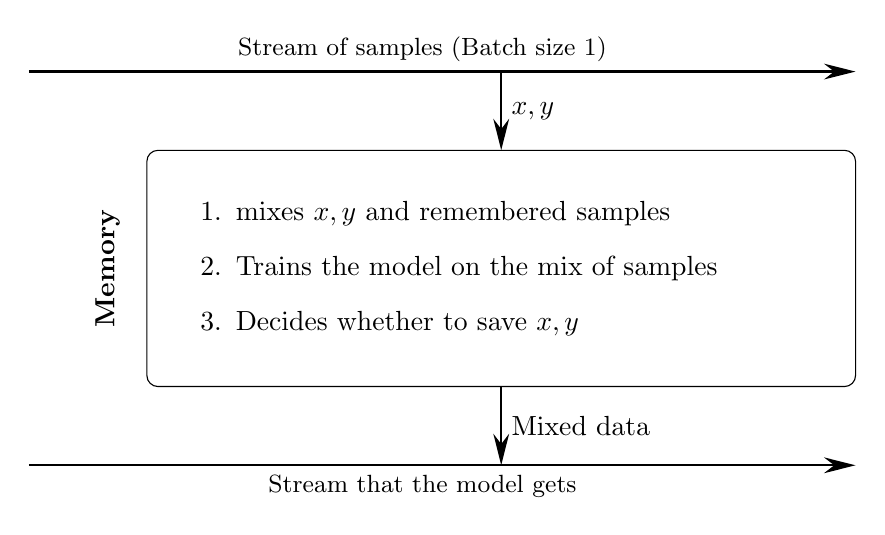
\begin{tikzpicture}[
    box/.style = {draw, rounded corners, minimum width=9cm, minimum height=3cm, align=center},
    arrow/.style = {thick, -{Stealth[length=4mm, width=2mm]}},
    textnode/.style = {font=\small}
]

% Draw top horizontal arrow over Memory label
\draw[arrow] (-6,2.5) -- (4.5,2.5);
\node[textnode, above] at (-1, 2.5) {Stream of samples (Batch size 1)};

% Memory label on the left, behind the arrows
\node[rotate=90, anchor=center] at (-5, 0) {\textbf{Memory}};

% Vertical arrow down to box with label x,y
\draw[arrow] (0,2.5) -- (0,1.5) node[right, pos=0.5] {$x, y$};

% Box for algorithm block
\node[box] (memory) at (0,0) {\begin{minipage}{8.5cm}
\begin{enumerate}
  \item mixes $x, y$ and remembered samples\;
  \item Trains the model on the mix of samples
  \item Decides whether to save $x, y$\;
\end{enumerate}

\end{minipage}};

% Vertical arrow down from box with label Mixed data
\draw[arrow] (0,-1.5) -- (0,-2.5) node[right, pos=0.5] {Mixed data};

% Bottom horizontal arrow
\draw[arrow] (-6,-2.5) -- (4.5,-2.5);
\node[textnode, below] at (-1, -2.5) {Stream that the model gets};

\end{tikzpicture}
\caption{Experience Replay streaming pipeline}
\label{fig:memory-stream}
\end{figure}

Now that we described how Backpropagation and Experience replay work we will explain how the specific memory modules we experimented with work.

\subsection{Experience Replay-Method (ER-M)}
The simplest method, used a lot as a baseline gets it's name directly from the method it uses, ER-M doesn't try to do anything smart, it just saves samples at random and mixes them the same. Although, the way it saves samples is based soley on randomness it does sample it in a special way called reservoir sampling that ensures that from a stream of data the chance for every sample to be in memory is uniform, unlike classic random sampling where older samples have a bigger chance of being overwritten. As it doesn't have to calculate much this is regarded as one of the fastest methods and it performs quite well. The algorithm for which looks as so:
\begin{algorithm}[t]
\SetKwFunction{ReservoirSample}{ReservoirSample}
\SetKwInOut{Input}{Input}
\SetAlgoNoEnd

\Input{Memory $\mathbf{M}$, Sample $\mathbf{}{S}$, MaxSize $ \mathbf{K} $}
\Input{(Optional Weight of Sample $\mathbf{W}$)}

  $r \leftarrow \text{random}()^ {1/W} $ \tcp*{\textit{uniform (0, 1]}}
  \If{$M.\text{Count} < K$}{
    $M.\text{Insert}(r, S)$\;
  }
  \Else{
    \If{$r > M.\text{Minimum}$}{
      $M.Argmin \leftarrow (r, S)$\;
    }
  }

\caption{Reservoir sampling using min-priority queue}
\label{alg:reservoir}
\end{algorithm}

ER-M's strategy for mixing samples into the data stream is to make a batch of a random sample from it's memory and a incoming sample, then pass this to the model to train on.

\subsection{Gradient Sample Selection (GSS)}

An earlier though more complex method devised is called \textbf{Gradient Sample Selection (GSS)}, which maximizes the difference of angles between the model's update gradients for each sample saved. This is motivated by the expectation that if the all the gradients point in a different direction it will lead to good generalization, as well as a good class distribution in the memory. The algorithm for it looks like this:

\begin{algorithm}[H]
\SetKwFunction{GSS}{GSS}
\SetKwInOut{Input}{Input}
\SetAlgoNoEnd

\Input{Memory $\mathbf{M}$, Sample $\mathbf{S}$, MaxSize $\mathbf{K}$}
\Input{Threshold $\mathbf{T}$, Sampling Count $C$, Model}

$Subset \leftarrow M.\text{Choice}(C)$ \\
$Gradients \leftarrow \text{Model.CalculateGradients}(Subset)$ \\
$Gradient \leftarrow \text{Model.CalculateGradients}(S)$ \\
$similarities \leftarrow \text{CosineSimilarity}(Gradients, Gradient)$ \\

\If{$\max(similarities) < T$}{
    $Candidates \leftarrow M.\text{Choice}(|S|, M.similarities)$ \tcp*{\textit{M.similarities is the distribution}}
    
    \For{$(c, s) \in \text{zip}(Candidates, S)$}{
        $r \sim \mathcal{U}(0, 1)$ \\
        \If{$r < \frac{c.sim}{c.sim + s.sim}$}{
            $M.\text{replace}(c, s)$
        }
    }
}

\caption{GSS Memory Update}
\label{alg:reservoir}
\end{algorithm}
Here when mixing the data, it's default configuration trains on every given sample 10 times, between every sample it mixes 10 batches selected by random from the memory. So (x, y) -> (x,y),(rand batch 1),(x,y)(rand batch 2) ...

\subsection{Dark Experience Replay ++ (DER++)} 
DER++ works the same as ER-M in the way it decides which samples to save, but as an added bonus it saves the model's whole output, even if it's not completely correct, the motivation behind this is to not keep reteaching the model the correct behavior, but also it's original behavior as well, What it does differently is it calculates one loss for each sample that consists of three parts, the incoming sample loss, a mean squared loss in respect to it's original prediction and again a normal loss for a sample from the memory, the later two losses are multiplies by two hyperparameters, $\alpha$ and $\beta$ respectively(both are usually set to 0.5).

\chapter{Experiments}

We implemented our scenario using 3 different datasets, Mnist, CIFAR10 and CIFAR100 for which we implemented 3 different protocols to test and show where the tested methods fail.
Those being
\begin{itemize}
    \item \textbf{I.I.D.} is a typical run on a dataset
    \item \textbf{Disjoint} splits the dataset into multiple tasks containing only a number of classes, which are run sequentially
    \item \textbf{Weave} splits the dataset the same as Disjoint, but the task is built up out of threads of a given length that are constructed by picking a random sample in the task and iteratively finding it's closest neighbor in the DINOv2~\cite{DINOv2} embedding space. We used a thread length of 16.
    % \item \textbf{Disjoint Permuted} is split like disjoint, but every task is given through a random permutation 
\end{itemize}

\section{General}
Here we test a subset of state of the art methods being GSS, ER, DER++ in our scenario with a batch size of one and only a single pass of the dataset. To stay true to the field's baseline model if not stated otherwise we ran all the experiments on the ResNet18 architecture with the modification of removing the batch normalization as makes no sense with our chosen batch size. The optimizer used was SGD~\cite{SGD} with a fixed learning rate of 0.0005 which has to be smaller than typical due to the batch size of one. As we test on a fairly nontrivial dataset(CIFAR100) we decided the memory size should reflect this, leading to us choosing a fixed size of 1000 samples. The default scenario we test on is Disjoint CIFAR10 as it is a nice balance between Mnist(too easy) and CIFAR100(too hard).

To show how the methods behave we plot their task-wise accuracies with respect to time. Another two plot's we have available is of the memory's class distribution and the share of data the model is learning from at each moment. 

The first experiment we performed is a study of the overall performance of the base implementations of each method across the Disjoint and Weave scenario for every dataset. The results can be seen in \hyperref[tab:overall_accuracy]{Table 4.1}. 

\begin{table}[t]
    \centering
    \caption{Accuracies of base implementations on different dataset scenarios}
    \label{tab:overall_accuracy}
    \begin{tabular}{lcccccc}
        \toprule
        & \multicolumn{2}{c}{\textbf{MNIST}} & \multicolumn{2}{c}{\textbf{CIFAR10}} & \multicolumn{2}{c}{\textbf{CIFAR100}} \\
        & Disjoint & Weave & Disjoint & Weave & Disjoint & Weave \\
        \midrule
        \textbf{I.I.D.}    & \multicolumn{2}{c}{97.5} & \multicolumn{2}{c}{46.8} & \multicolumn{2}{c}{19.8} \\
        \arrayrulecolor{gray!80}
        \midrule
        \arrayrulecolor{black} 
        \textbf{No Memory} & 19.8 & 19.9 & 18.4  & 16.3  & 7.5  & 1.0 \\
        \textbf{GSS}       & 85.4 & 87.7 & 32.2  & 26.7  & 5.4  & 4.2 \\
        \textbf{ER}        & 95.7 & 95.9 & 34.8  & 29.3  & 5.4  & 4.8 \\
        \textbf{DER++}     & 85.5 & 85.2 & 27.1  & 23.5  & 11.8 & 8.5 \\
        \bottomrule
    \end{tabular}
\end{table}

As a starting point for our deeper investigations, we performed an ablation study of GSS's hyperparameters, those being NUM\_ITERS(the number of times it train's on a incoming sample), SAMPLE\_COUNT(the amount of samples from the memory it uses to gauge the gradient similarity) and THRESHOLD(The threshold of when to replace a sample in memory). From the result's seen in \hyperref[tab:gss-ablation]{Table 4.2} we concluded that increasing NUM\_ITERS had the biggest positive impact on accuracy and that the a negative threshold has a big impact in the other direction.

\begin{table}[t]
\centering
\caption{Ablation study on GSS hyperparameters for CIFAR-10. Results are reported as classification accuracy (\%).}
\label{tab:gss-ablation}
\begin{tabular}{ccc|c}
\toprule
\textbf{NUM\_ITERS} & \textbf{SAMPLE\_COUNT} & \textbf{THRESHOLD} & \textbf{Accuracy (\%)} \\
\midrule
10 & 10 & 0.0 & 32.2 (Default) \\
\arrayrulecolor{gray!80}
\midrule
\arrayrulecolor{black} 
5    & --   & --   & 33.7 \\
15    & --   & --   & \textbf{38.5} \\
\arrayrulecolor{gray!80}
\midrule
\arrayrulecolor{black} 
--    & 5   & --   & \textbf{35.1} \\
--    & 15   & --   & 32.3 \\
\arrayrulecolor{gray!80}
\midrule
\arrayrulecolor{black} 
--    & --   & -0.1   & 26.9 \\
--    & --   & 0.1   & \textbf{31.1} \\
\bottomrule
\end{tabular}
\end{table}

The rest  will divide our experiments into three different approaches: \textbf{\hyperref[sec:expone]{GSS Memory Management}, \hyperref[sec:exptwo]{General Improvements}} and \textbf{\hyperref[sec:expthree]{Pre training}}

\section{GSS Memory Management}
\label{sec:expone}
This section came from us noticing that the mechanism for saving samples into the memory in GSS is quite complex. We wanted to test out if we could come up with a way to improve it.

\subsection{Forcing uniform class distribution}
We noticed that the task-wise distribution of samples in the memory is very biased to the first task. That lead us to a hypothesis that if we equalize this distribution it would lead to better performance. To see if that is the case we added a mechanism that checks if the class of an incoming sample is not yet in the memory. If it isn't, we calculate the amount of memory that should be allocated to each class by dividing the memory size by the number of classes encountered. We then keep only this amount of every class, throwing out any extra, ordering them by their gradient angle similarity to stay true the original method.
As seen in \hyperref[fig:gss-cifar10-grid]{Figure 4.1} the performance on the first task diminished but increased for every other task, though not enough to make a significant difference. 

\begin{figure}[t]
    \centering
    \begin{subfigure}[t]{0.48\linewidth}
        \centering
        \includegraphics[width=\linewidth]{figures/DISJOINT2_GSS1k_B1_accuracy.png}
        \label{fig:gss-cifar10-accuracy}
    \end{subfigure}
    \hfill
    \begin{subfigure}[t]{0.48\linewidth}
        \centering
        \includegraphics[width=\linewidth]{figures/DISJOINT2_GSS1k_B1_memory.png}
        \label{fig:gss-cifar10-fe-accuracy}
    \end{subfigure}
    \begin{subfigure}[t]{0.48\linewidth}
        \centering
        \includegraphics[width=\linewidth]{figures/DISJOINT2_GSS1k_B1_FORCED_EQUALITY_accuracy.png}
        \label{fig:gss-cifar10-mem-share}
    \end{subfigure}
    \hfill
    \begin{subfigure}[t]{0.48\linewidth}
        \centering
        \includegraphics[width=\linewidth]{figures/DISJOINT2_GSS1k_B1_FORCED_EQUALITY_memory.png}
        \label{fig:gss-cifar10-fe-mem-share}
    \end{subfigure}

    \caption{Comparison of GSS results on CIFAR-10: top row = accuracy, bottom row = memory share. Left = original GSS, right = forced equality variant.}
    \label{fig:gss-cifar10-grid}
\end{figure}

\subsection{Filling with a threshold}
Two things we noticed, were that when the memory is getting filled up it does so with data not optimized based on the gradient angle and that saved examples almost never get replaced by examples of the same class. This lead us to the hypothesis that if we fill up the memory with examples optimized with the GSS's metric the performance would increase. To do so we added the threshold filter to the filling stage, which was supposed to ensure the examples saved would have a similarity of less than the threshold.

Although as can be seen in \hyperref[fig:gss-fill-threshold-comparison]{Figure 4.2} there is a problem with our approach, as if we keep the threshold at the default value of 0 the memory isn't able to fill and if we increase it to a level where it would fill(0.3) the old samples get replaced too easily. 

\begin{figure}[t]
    \centering
    \begin{subfigure}[t]{0.48\linewidth}
        \centering
        \includegraphics[width=\linewidth]{figures/DISJOINT_GSS1k_B1_FILL_WITH_THRESHOLD_memory.png}
        \label{fig:gss-fill-0}
    \end{subfigure}
    \hfill
    \begin{subfigure}[t]{0.48\linewidth}
        \centering
        \includegraphics[width=\linewidth]{figures/DISJOINT_GSS1k_B1_THRESHOLD_0.3_FILL_WITH_THRESHOLD_memory.png}
        \label{fig:gss-fill-0.3}
    \end{subfigure}

    \caption{Comparison of GSS fill behavior with threshold 0 (left) and threshold 0.3 (right).}
    \label{fig:gss-fill-threshold-comparison}
\end{figure}

\subsection{Weighted Reservoir}
It seemed to us that GSS's mechanism to save examples to the memory, could be improved upon. So we wanted to see what would happen if we took reservoir sampling, which has good task-wise memory distribution and modified it by adding GSS's similarity score as a weight to the random sampling. This would show us if the gradient metric makes sense or not.

As can be seen in \hyperref[fig:reservoir-grad-angle]{Figure 4.3} there is a noticeable difference, not in overall performance, but more in the way the model remembers the data. We theorize that GSS's metric really does lead to better generalization, but it still isn't enough to solve the problem of catastrophic forgetting, we study ways to do so in the section \hyperref[sec:exptwo]{General Improvements}

\begin{figure}[t]
    \centering
    \begin{subfigure}[t]{0.48\linewidth}
        \centering
        \includegraphics[width=\linewidth]{figures/CIFAR10_DISJOINT_RESERVOIR_accuracy.png}
        \label{fig:gss-fill-0}
    \end{subfigure}
    \hfill
    \begin{subfigure}[t]{0.48\linewidth}
        \centering
        \includegraphics[width=\linewidth]{figures/CIFAR10_DISJOINT_RESERVOIR_GRAD_ANGLE_accuracy.png}
        \label{fig:gss-fill-0.3}
    \end{subfigure}

    \caption{Comparison of task-wise accuracy between ER(left) and ER-Weighted(right).}
    \label{fig:reservoir-grad-angle}
\end{figure}

\section{General Improvements}
\label{sec:exptwo}
In this section we aim to test any general improvements we could make to the methods that we have chosen.

\subsection{GSS and ER with 10 training iterations per sample}
Starting off \hyperref[tab:gss-ablation]{Table 4.2} inspired us to test if introducing NUM\_ITERS at a value of 10 to the other methods would increase their performance as it does with GSS. The difference in performance was negligible for ER and even negative by 3\% for DER++. We realized that by doing this it has a similar effect as simply increasing the learning rate.

\subsection{Augmentations}
As an improvement to this we wanted to test weather adding augmentations to the methods would have an have any positive effects and if combining this with the increase in NUM\_ITERS would work even better. As can be seen in \hyperref[tab:augment-comparison]{Table 4.3} the combination worked wonders for GSS and ER, sadly not for DER++.

\begin{table}[t]
\centering
\caption{Comparison of methods with augmentations and NUM\_ITERS variants. TODO}
\label{tab:augment-comparison}
\begin{tabular}{lccc}
\toprule
& \textbf{GSS} & \textbf{ER} & \textbf{DER++} \\
\midrule
Base & 32.2 & 34.8 & 27.1 \\
Augmented & -- & 28.9 & 17.7 \\
Both & 40.1 & 43.2 & 24.7 \\
\bottomrule
\end{tabular}
\end{table}

\begin{figure}[t]
    \centering
    \begin{subfigure}[t]{0.48\linewidth}
        \centering
        \includegraphics[width=\linewidth]{figures/CIFAR10_DISJOINT_RESERVOIR_accuracy.png}
    \end{subfigure}
    \hfill
    \begin{subfigure}[t]{0.48\linewidth}
        \centering
        \includegraphics[width=\linewidth]{figures/CIFAR10_DISJOINT_RESERVOIR_shares.png}
    \end{subfigure}

    \begin{subfigure}[t]{0.48\linewidth}
        \centering
        \includegraphics[width=\linewidth]{figures/CIFAR10_DISJOINT_RESERVOIR_EQUAL_SAMPLING_accuracy.png}
    \end{subfigure}
    \hfill
    \begin{subfigure}[t]{0.48\linewidth}
        \centering
        \includegraphics[width=\linewidth]{figures/CIFAR10_DISJOINT_RESERVOIR_EQUAL_SAMPLING_shares.png}
    \end{subfigure}

    \caption{Task-wise accuracy and training share of ER(top) and ER with Equal sampling(bottom) on Disjoint CIFAR10}
    \label{fig:er-equal-sampling}
\end{figure}

\subsection{Equal Sampling}
Another thing we realized when looking at the task-wise accuracy of ER in \hyperref[fig:er-equal-sampling]{Figure 4.3} is that it falls almost instantly and then gradually if at all climbs back up. This inspired the thought that this behavior could be caused by how the memorized samples are mixed into the training stream.

Once we looked at the task-wise training data shares in \hyperref[fig:er-equal-sampling]{Figure 4.3} we saw that it required balancing, as in the worst case scenario for a classification problem of ten tasks. One class can have six times the chance to be in the stream then other classes. We propose a strategy where for every one sample incoming, we mix in samples from every other class. For example if we are in a ten class problem and our memory already contains all ten classes if we get an example from class ten, our method will instead of just mixing in one other random example, mix in nine different examples, one for every class one through nine.

This mixing strategy has a downside that should be pointed out, it being that it's speed doesn't scale well to higher order classification problems, due to it creating a batch the size of the count of every unique class in memory.

As can be seen in \hyperref[fig:er-equal-sampling]{Figure 4.3}, our method of equal sampling improves on the instant catastrophic forgetting, although the model still does end up forgetting the previous tasks. We believe this is due to the model overfitting to the samples in the memory which is something augmentations can help with.

\subsection{Zero Aberation A Zillion Augmentations Mixing (ZAAZA-Mix)}
Here we combine the findings we have made into one method. We show it as a modification to ER, but it can be used for any experience replay method. It consists of mixing an equal amount of every class into one batch, then augmenting it and training the model with it. This is done NUM\_ITERS times for every incoming sample. The algorithm for it is described in \hyperref[alg:ZAAZA-Mix]{Algorithm 4}. This method improves the model's accuracy by quite a large margin of 12\%, as can be seen in \hyperref[fig:er-zaaza]{Figure 4.5}. It does this by lifting up the overall accuracy of past tasks, however it is not able to learn the current task as well as for example ER, still overall it achieves better performance on our single-pass batch size one scenario.

\begin{figure}[t]
    \centering
    \begin{subfigure}[t]{0.48\linewidth}
        \centering
        \includegraphics[width=\linewidth]{figures/CIFAR10_DISJOINT_RESERVOIR_BASE_accuracy.png}
    \end{subfigure}
    \hfill
    \begin{subfigure}[t]{0.48\linewidth}
        \centering
        \includegraphics[width=\linewidth]{figures/CIFAR10_DISJOINT_ZAAZA_accuracy.png}
    \end{subfigure}

    \caption{Task-wise accuracy of ER(left) and ER with ZAAZA-Mix}
    \label{fig:er-zaaza}
\end{figure}



\begin{algorithm}[t]
\label{alg:ZAAZA-Mix}
\SetAlgoLined
\KwIn{Data stream $S$}
\KwOut{Updated model and memory}

\While{samples remain in $S$}{
    sample $\gets$ \texttt{pop}$(S)$\;
    \For{$i \gets 1$ \KwTo NUM\_ITER}{
        batch $\gets$ \{sample\}\;

        \ForEach{class $\in$ Memory}{
            \If{class $\neq$ sample.class}{
                batch $\gets$ batch $\cup$ \texttt{randomChoice}$(\text{Memory[class]})$\;
            }
        }
        augmentedBatch $\gets$ \texttt{augment}$(\text{batch})$\;
        model.step(augmentedBatch)\;
    }
    memory.observe(sample)\;
}
\caption{Online Learning with Memory and Augmentation}
\end{algorithm}

\section{Pre-training}
\label{sec:expthree}
Normally when training a model it is run for multiple epochs, because one epoch even if it is i.i.d. it will not produce a very good model. This can be seen very clearly on the the CIFAR100 dataset, which is more complex of a classification task then CIFAR10 or Mnist. As we are interested in the scenario with only a single pass of the dataset, there is little chance a creating a great classification model.

To tackle this problem there is a method of using a powerful pretrained model and then adding a couple layers to the end and only training those. This has the benefit of having a great model for feature extraction and still the plasticity of the few layers to mold it to our problem. Here we test how using a very powerful self-supervised model react to training in our scenario.

The pretrained model we used is DINOv2 small from meta research labs, which accepts an input image of 224x224 and returns a feature vector in an embeding space of 384 dimensions. We then add three fully connected layers to it(384->256->128->NUM\_CLASSES), these being the only part of it we train.

As can be seen in \hyperref[tab:pre-training-comparison]{Table 4.4} the accuracies are vastly better than our best result's using a ResNet18 Model. This method can be used to make a model that is very capable and can be used in real world scenarios, where a \~40\% accuracy is not good enough, let alone \~10\% on CIFAR100.

This method does have a downside, that being that it requires to have a pre-trained a model on a problem at least similar to what is expect of it to learn, this is why we chose a self-supervised model, as it can sometimes generalize better and requires less work in compiling the dataset for it's training~\cite{self-supervized-generalization}. For explanation a model trained on classifying numbers, will output a close to meaningless embedding if given an image of a car.

\begin{table}[t]
    \centering
    \caption{Accuracies of base implementations on different dataset scenarios}
    \label{tab:pre-training-comparison}
    \begin{tabular}{lcccc}
        \toprule
        & \multicolumn{2}{c}{\textbf{ResNet18}} & \multicolumn{2}{c}{\textbf{DINOv2+Fc}} \\
        & ER & ZAAZA & ER & ZAAZA \\
        \midrule
        \textbf{I.I.D.}   & \multicolumn{2}{c}{19.8} & \multicolumn{2}{c}{81.9} \\
        \arrayrulecolor{gray!80}
        \midrule
        \arrayrulecolor{black} 
        \textbf{Disjoint} & 5.4 & 10.6 & 68.4 & -- \\
        \textbf{Weave}  & 4.8 & 9.5  & 66.3 & -- \\
        \bottomrule
    \end{tabular}
\end{table}












\chapter{Discussion}

This thesis set out to investigate though empirical examination a subset of OCL methods and see how they work in the modified scenario inspired by our interest in biological plausible machine learning. We succeeded in implementing and examining three methods(GSS, ER and DER++), that fall into the scope of the scenario we created. 
A summary for the findings respective to each method are:
\begin{itemize}
    \item DER++ performed worse than our expectations based on the original paper, likely due to their nonconformance to OCL's criteria of a single pass of the dataset, as in the original paper expands each task for CIFAR10 by 50 times.
    \item GSS's mechanism for saving examples into memory doesn't ensure a good distribution among tasks/classes, as it depends a lot on what the dataset looks like with respect to model updates. However it's introduction of training multiple times for every incoming sample is a good practice and noticeably improves a models performance. 
    \item ER is a simple method to implement and has the same task/class distribution as the whole dataset stream. It performs quite well and makes for a great baseline or base model to build upon as seen in DER++, MIR or our proposed method. 
\end{itemize}
Our empirical experimentation inspired several key contributions to OCL. First of which being our proposed method ZAAZA, that focuses on the importance of transforming the incoming non-i.i.d. stream to it's ...(opposite). By heavily augmenting the samples before the model trains on them and ensuring the class distribution is uniform through creating batches with one of every class for each incoming sample.

Second, being the experimentation of using pre-trained embedding models as a way to simplify the problem, thus shortening the time to learn a given task. We did this with the use of DINOv2 a self-supervised vision embedding model. It's property of being trained in a self-supervised manner is a nice bonus to our motivation of biological plausibility~\cite{brain-self-supervised}.

Third, we introduced another benchmark to OCL, that being the Weave scenario which was created to impede the learning ability of typical machine learning processes even more than the Disjoint scenario.

While we believe the original goals of this thesis have been fulfilled, there are some shortcomings to be acknowledged, most of which can be attributed to time limitations. For instance we we're not able to go as in depth as we would have liked in some of our experiments, which would have reduced the possibility of certain subtleties of the chosen methods being missed. Additionally we would have liked to implement and experiment with more then the three methods we did, for example RM~\cite{RM} and AQM~\cite{AQM}. We would have also liked to flesh out our idea of the weighted reservoir, perhaps testing it with other metrics for example RM's.

In future work we would like to tackle these shortcoming and flesh out our proposals in more detail. 

In conclusion this thesis has explored the space of OCL through research of the state of the art and empirical study and successfully improved upon some of the methods.

\appendix

\chapter{Appendix}

\subsection{Learning only from memory}
When setting up one of the experiments we accidentally stumbled on learning only from the memory, this worked fairly well and helped in inspiring our proposed equal mixing method. However even though the results that can be seen in \hyperref[fig:only-mem-zaza]{Figure A.1} are quite good It is a very inefficient use of the data and as we has been showed better performance is achieved when mixing in the current data. We theorize that this is method shows the best performance that can be possibly gotten from the subset saved in the memory, without any major improvement's to the underlying learning mechanism(Regularization/Architecture...)
\begin{figure}[h]
    \centering
    \includegraphics[width=0.75\linewidth]{figures/CIFAR10_DISJOINT_ZAAZA_ONLY_MEMORY_accuracy.png}
    \caption{Training accuracy of ZAAZA on Disjoint CIFAR10 learning only from memory}
    \label{fig:only-mem-zaza}
\end{figure}

\subsection{Weave scenario}
In this section we delve deeper into our motivations behind and expectations of the Weave scenario we propose. It is motivated by our realization that in a typical Disjoint scenario although it is in it's entirety non-i.i.d. the tasks of which it's made of are i.i.d. This means that inside a task the model learns it in a very typical way. Our Weave scenario tries to combat this by ensuring that the inside of each task is not entirely i.i.d., by building it out of thread of a given length that are a collection of images similar to each other. 

In our example we use the distance of two images in the DINOv2 embedding space as the similarity metric, but this can be switched out for any other metric, based on the data being trained on. A naive and slow algorithm for creating the scenario can be seen in \hyperref[alg:weave]{Algorithm 5}.

As a bonus the i.i.d.-ness can be controlled by the thread length, setting it higher means it will make the scenario less i.i.d than with a lower length, due to the increased length in which the model will rather overfit than generalize. 

A collection of these threads form CIFAR10 can be seen in \hyperref[fig:weave]{Figure A.2}
\begin{algorithm}[h]
\SetAlgoLined
\KwIn{Pools of images $\mathcal{P} = \{\mathcal{P}_1, \ldots, \mathcal{P}_T\}$, number of tasks $T$, thread length $K$}
\KwOut{Disjoint tasks $\{\mathcal{T}_1, \ldots, \mathcal{T}_T\}$ composed of similarity threads}

\For{$t \gets 1$ \KwTo $T$}{
    % Compute embeddings for all images in current pool using DINOv2
    Compute embeddings for all samples in $\mathcal{P}_t$ using DINOv2\;
    
    Initialize task: $\mathcal{T}_t \gets \emptyset$\;
    
    % Initialize first thread by randomly popping a sample from the pool
    thread $\gets$ \texttt{popRandom}($\mathcal{P}_t$)\;
    
    \While{$\mathcal{P}_t$ is not empty}{
        % If thread reached the desired length, finalize it and start a new one
        \If{$|$thread$| \geq K$}{
            $\mathcal{T}_t \gets \mathcal{T}_t \cup \text{thread}$\;
            thread $\gets$ \texttt{popRandom}($\mathcal{P}_t$)\;
        }
        
        % Find and remove the closest neighbor to the last element in the current thread
        neighbor $\gets$ \texttt{popClosest}(\text{last}(thread), $\mathcal{P}_t$)\;
        
        % Add the neighbor to the current thread
        thread $\gets$ thread $\cup$ \{neighbor\}\;
    }
    
    % Add the last thread if it has any samples remaining
    \If{$|$thread$| > 0$}{
        $\mathcal{T}_t \gets \mathcal{T}_t \cup \text{thread}$\;
    }
}

\caption{Constructing the Weave Scenario via Similarity Threads}
\label{alg:weave}
\end{algorithm}

\begin{figure}[h]
    \centering
    \includegraphics[width=1\linewidth]{figures/weave.png}
    \caption{Example of threads created in our Weave scenario from CIFAR10}
    \label{fig:weave}
\end{figure}

\bibliographystyle{plain}
\bibliography{ctuman-mwe}

\end{document}

